\documentclass[14pt, a4paper]{extarticle}

\usepackage[margin=1in]{geometry}
\usepackage{graphicx}
\usepackage{enumitem}
\usepackage{multicol}
\usepackage{fancyhdr}
\usepackage{amsfonts}
\usepackage{amssymb}
\usepackage{listings}
\usepackage{float}
\usepackage{wrapfig}

\usepackage{gvv-book}
\usepackage{gvv}

\graphicspath{ {figs/} }

\pagestyle{fancy}
\fancyhf{} 
\fancyhead[L]{2017}
\fancyhead[R]{PH}
\fancyfoot[L]{PH}
\fancyfoot[R]{\thepage/13}
\renewcommand{\headrulewidth}{0.4pt}
\renewcommand{\footrulewidth}{0.4pt}

\let\oldvec\vec
\renewcommand{\vec}[1]{\overrightarrow{#1}}
\newcommand{\myvec}[1]{\begin{bmatrix} #1 \end{bmatrix}}

\begin{document}

\begin{center}
    \Large\textbf{GATE Physics 2017 Question Paper}
\end{center}

\noindent\textbf{Q. 1 – Q. 25 carry one mark each.}
\hrule

\begin{enumerate}[label=\textbf{Q.\arabic*}]

\item Identical charges $q$ are placed at five vertices of a regular hexagon of side $a$. The magnitude of the electric field and the electrostatic potential at the centre of the hexagon are respectively
    \begin{enumerate}
        \item $0, 0$
        \item $\frac{q}{4\pi\epsilon_0 a^2}, \frac{q}{4\pi\epsilon_0 a}$
        \item $\frac{q}{4\pi\epsilon_0 a^2}, \frac{5q}{4\pi\epsilon_0 a}$
        \item $\frac{\sqrt{5}q}{4\pi\epsilon_0 a^2}, \frac{\sqrt{5}q}{4\pi\epsilon_0 a}$
    \end{enumerate}
    \hfill \textbf{(GATE PH 2017)}
    
    \item A parallel plate capacitor with square plates of side 1 m separated by 1 micro meter is filled with a medium of dielectric constant of 10. If the charges on the two plates are 1 C and -1 C, the voltage across the capacitor is \underline{\hspace{5em}} kV. (up to two decimal places). ($\epsilon_0 = 8.854 \times 10^{-12}\,\text{F/m}$)
    \hfill \textbf{(GATE PH 2017)}

\item Light is incident from a medium of refractive index $n=1.5$ onto vacuum. The smallest angle of incidence for which the light is not transmitted into vacuum is \underline{\hspace{3cm}} degrees. (up to two decimal places).
\hfill \textbf{(GATE PH 2017)}

\item A monochromatic plane wave in free space with electric field amplitude of 1 V/m is normally incident on a fully reflecting mirror. The pressure exerted on the mirror is \underline{\hspace{3cm}} $\times 10^{-12}$ Pa. (up to two decimal places) ($\epsilon_0 = 8.854 \times 10^{-12}$ F/m).
\hfill \textbf{(GATE PH 2017)}

\item The best resolution that a 7 bit A/D convertor with 5 V full scale can achieve is \underline{\hspace{3cm}} mV. (up to two decimal places).
\hfill \textbf{(GATE PH 2017)}

\item In the figure given below, the input to the primary of the transformer is a voltage varying sinusoidally with time. The resistor R is connected to the centre tap of the secondary. Which one of the following plots represents the voltage across the resistor R as a function of time?
\begin{figure}[H]
\centering
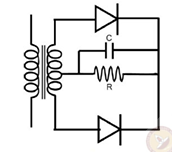
\includegraphics[width=0.4\textwidth]{figs/q6figA17.png}
\caption{circuit diagram}
\label{fig:q6_circuit}
\end{figure}
\begin{enumerate}
\begin{multicols}{2}
\item 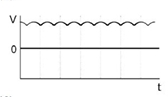
\includegraphics[width=\linewidth]{figs/q6figb17.png}
\item 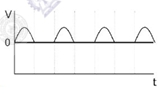
\includegraphics[width=\linewidth]{figs/q6figc7.png}
\item 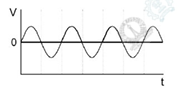
\includegraphics[width=\linewidth]{figs/q6figd17.png}
\item 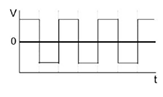
\includegraphics[width=\linewidth]{figs/q6fige17.png}
\end{multicols}
\end{enumerate}
\hfill \textbf{(GATE PH 2017)}

\item The atomic mass and mass density of Sodium are 23 and 0.968 g cm$^{-3}$, respectively. The number density of valence electrons is \underline{\hspace{3cm}} $\times 10^{22}$ cm$^{-3}$. (Up to two decimal places.) (Avogadro number, $N_A = 6.022 \times 10^{23}$).
\hfill \textbf{(GATE PH 2017)}

\item Consider a one-dimensional lattice with a weak periodic potential $U(x) = U_0 \cos\left(\frac{2\pi x}{a}\right)$. The gap at the edge of the Brillouin zone $\left(k = \frac{\pi}{a}\right)$ is:
\begin{enumerate}
\begin{multicols}{4}
\item $U_0$
\item $\frac{U_0}{2}$
\item $2U_0$
\item $\frac{U_0}{4}$
\end{multicols}
\end{enumerate}
\hfill \textbf{(GATE PH 2017)}

\item Consider a triatomic molecule of the shape shown in the figure below in three dimensions. The heat capacity of this molecule at high temperature (temperature much higher than the vibrational and rotational energy scales of the molecule but lower than its bond dissociation energies) is:
\begin{figure}[H]
\centering
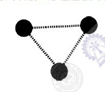
\includegraphics[width=0.2\textwidth]{figs/q9fig17.png}
\caption{triatomic molecule }
\label{fig:triatomic}
\end{figure}
\begin{enumerate}
\begin{multicols}{4}
\item $\frac{3}{2}k_B$
\item $3k_B$
\item $\frac{9}{2}k_B$
\item $6k_B$
\end{multicols}
\end{enumerate}

\item If the Lagrangian $L_0 = \frac{1}{2} m \left(\frac{dq}{dt}\right)^2 - \frac{1}{2} m \omega^2 q^2$ is modified to $L = L_0 + \alpha q \left(\frac{dq}{dt}\right)$, which one of the following is TRUE?
\begin{enumerate}
\item Both the canonical momentum and equation of motion do not change
\item Canonical momentum changes, equation of motion does not change
\item Canonical momentum does not change, equation of motion changes
\item Both the canonical momentum and equation of motion change
\end{enumerate}
\hfill \textbf{(GATE PH 2017)}

\item Two identical masses of 10 gm each are connected by a massless spring of spring constant 1 N/m. The non-zero angular eigenfrequency of the system is \underline{\hspace{3cm}} rad/s. (up to two decimal places).
\hfill \textbf{(GATE PH 2017)}

\item The phase space trajectory of an otherwise free particle bouncing between two hard walls elastically in one dimension is a
\begin{enumerate}
\begin{multicols}{4}
\item straight line
\item parabola
\item rectangle
\item circle
\end{multicols}
\end{enumerate}
\hfill \textbf{(GATE PH 2017)}

\item The Poisson bracket $[x, x p_y + y p_x]$ is equal to
\begin{enumerate}
\begin{multicols}{4}
\item $-x$
\item $y$
\item $2p_x$
\item $p_y$
\end{multicols}
\end{enumerate}
\hfill \textbf{(GATE PH 2017)}

\item The wavefunction of which orbital is spherically symmetric:
\begin{enumerate}
\begin{multicols}{4}
\item $p_x$
\item $p_y$
\item $s$
\item $d_{xy}$
\end{multicols}
\end{enumerate}
\hfill \textbf{(GATE PH 2017)}

\item The contour integral $\oint_C \frac{1}{1+z^2} dz$ evaluated along a contour going from $-\infty$ to $+\infty$ along the real axis and closed in the lower half-plane by a half circle is equal to \underline{\hspace{3cm}} (up to two decimal places).
\hfill \textbf{(GATE PH 2017)}

\item The Compton wavelength of a proton is \underline{\hspace{3cm}} fm. (up to two decimal places). ($m_p=1.67\times10^{-27}$ kg, $h=6.626\times10^{-34}$ Js, $e=1.602\times10^{-19}$ C, $c=3\times10^8$ ms$^{-1}$)
\hfill \textbf{(GATE PH 2017)}

\item Which one of the following conservation laws is violated in the decay $\tau^+ \to \mu^+ \mu^+ \mu^-$
\begin{enumerate}
\item Angular momentum
\item Total Lepton number
\item Electric charge
\item Tau number
\end{enumerate}
\hfill \textbf{(GATE PH 2017)}

\item Electromagnetic interactions are :
\begin{enumerate}
\item C conserving
\item C non-conserving but CP conserving
\item CP non-conserving but CPT conserving
\item CPT non-conserving
\end{enumerate}
\hfill \textbf{(GATE PH 2017)}

\item A one dimensional simple harmonic oscillator with Hamiltonian $H_0 = \frac{p^2}{2m} + \frac{1}{2} k x^2$ is subjected to a small perturbation, $H_1 = \alpha x + \beta x^3 + \gamma x^4$. The first order correction to the ground state energy is dependent on
\begin{enumerate}
\begin{multicols}{4}
\item only $\beta$
\item $\alpha$ and $\gamma$
\item $\alpha$ and $\beta$
\item only $\gamma$
\end{multicols}
\end{enumerate}
\hfill \textbf{(GATE PH 2017)}

\item For the Hamiltonian $H=a_0 I + \vec{b} \cdot \vec{\sigma}$ where $a_0 \in R$, $\vec{b}$ is a real vector, I is the $2\times2$ identity matrix, and $\vec{\sigma}$ are the Pauli matrices, the ground state energy is
\begin{enumerate}
\begin{multicols}{4}
\item $|b|$
\item $2a_0 - |b|$
\item $a_0 - |b|$
\item $a_0$
\end{multicols}
\end{enumerate}
\hfill \textbf{(GATE PH 2017)}

\item The coefficient of $e^{ikx}$ in the Fourier expansion of $u(x)=A \sin^2(\alpha x)$ for $k=-2\alpha$ is
\begin{enumerate}
\begin{multicols}{4}
\item $A/4$
\item $-A/4$
\item $A/2$
\item $-A/2$
\end{multicols}
\end{enumerate}
\hfill \textbf{(GATE PH 2017)}

\item The degeneracy of the third energy level of a 3-dimensional isotropic quantum harmonic oscillator is
\begin{enumerate}
\begin{multicols}{4}
\item 6
\item 12
\item 8
\item 10
\end{multicols}
\end{enumerate}
\hfill \textbf{(GATE PH 2017)}

\item The electronic ground state energy of the Hydrogen atom is $-13.6$ eV. The highest possible electronic energy eigenstate has an energy equal to
\begin{enumerate}
\begin{multicols}{4}
\item 0
\item 1 eV
\item +13.6 eV
\item $\infty$
\end{multicols}
\end{enumerate}
\hfill \textbf{(GATE PH 2017)}

\item A reversible Carnot engine is operated between temperatures $T_1$ and $T_2$ ($T_2>T_1$) with a photon gas as the working substance. The efficiency of the engine is
\begin{enumerate}
\begin{multicols}{4}
\item $1 - \frac{3T_1}{4T_2}$
\item $1 - \frac{T_1}{T_2}$
\item $1 - \left(\frac{T_1}{T_2}\right)^{3/4}$
\item $1 - \left(\frac{T_1}{T_2}\right)^{4/3}$
\end{multicols}
\end{enumerate}
\hfill \textbf{(GATE PH 2017)}

\item In the nuclear reaction $^{13}C_6 + \nu_e \to ^{13}N_7 + X$, the particle $X$ is
\begin{enumerate}
\begin{multicols}{2}
\item an electron
\item an anti-electron
\item a muon
\item a pion
\end{multicols}
\end{enumerate}
\hfill \textbf{(GATE PH 2017)}

\item Three charges (2 C, -1 C, -1 C) are placed at the vertices of an equilateral triangle of side 1m as shown in the figure. The component of the electric dipole moment about the marked origin along the $\hat{y}$ direction is \underline{\hspace{3cm}} C m.
\begin{figure}[H]
\centering
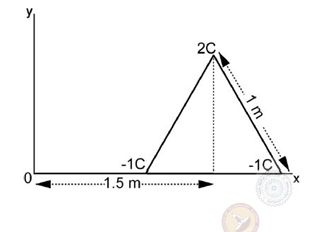
\includegraphics[width=0.4\textwidth]{figs/q26fig17.png}
\caption{charges on equilateral triangle}
\label{fig:q26}
\end{figure}
\hfill \textbf{(GATE PH 2017)}

\item An infinite solenoid carries a time varying current $I(t) = A t^2$, with $A \neq 0$. The axis of the solenoid is along the $\hat{z}$ direction. $\hat{r}$ and $\hat{\theta}$ are the usual radial and polar directions in cylindrical polar coordinates. $\vec{B} = B_r \hat{r} + B_{\theta} \hat{\theta} + B_z \hat{z}$ is the magnetic field at a point outside the solenoid. Which one of the following statements is true?
\begin{enumerate}
\begin{multicols}{2}
\item $B_r=0, B_{\theta}=0, B_z=0$
\item $B_r \neq 0, B_{\theta} \neq 0, B_z=0$
\item $B_r \neq 0, B_{\theta} \neq 0, B_z \neq 0$
\item $B_r=0, B_{\theta} \neq 0, B_z=0$
\end{multicols}
\end{enumerate}
\hfill \textbf{(GATE PH 2017)}

\item A uniform volume charge density is placed inside a conductor (with resistivity $10^{-2} \Omega$ m). The charge density becomes 1/(2.718) of its original value after time \underline{\hspace{3cm}} femto seconds. (up to two decimal places) ($\epsilon_0 = 8.854 \times 10^{-12}$ F/m)
\hfill \textbf{(GATE PH 2017)}

\item Water freezes at $0^{\circ}$C at atmospheric pressure ($1.01 \times 10^5$ Pa). The densities of water and ice at this temperature and pressure are 1000 kg/m$^3$ and 934 kg/m$^3$ respectively. The latent heat of fusion is $3.34 \times 10^5$ J/kg. The pressure required for depressing the melting temperature of ice by $10^{\circ}$C is \underline{\hspace{3cm}} GPa. (up to two decimal places)
\hfill \textbf{(GATE PH 2017)}

\item The minimum number of NAND gates required to construct an OR gate is:
\begin{enumerate}
\begin{multicols}{4}
\item 2
\item 4
\item 5
\item 3
\end{multicols}
\end{enumerate}
\hfill \textbf{(GATE PH 2017)}

\item Consider a 2-dimensional electron gas with a density of $10^{19}$ m$^{-2}$. The Fermi energy of the system is \underline{\hspace{3cm}} eV (up to two decimal places). ($m_e=9.31\times10^{-31}$kg, $h=6.626\times10^{-34}$Js, $e=1.602\times10^{-19}$C)
\hfill \textbf{(GATE PH 2017)}

\item The total energy of an inert-gas crystal is given by $E(R) = \frac{0.5}{R^{12}} - \frac{1}{R^6}$ (in eV), where R is the inter-atomic spacing in Angstroms. The equilibrium separation between the atoms is \underline{\hspace{3cm}} Angstroms. (up to two decimal places).
\hfill \textbf{(GATE PH 2017)}

\item Consider $N$ non-interacting, distinguishable particles in a two-level system at temperature $T$. The energies of the levels are 0 and $\varepsilon$, where $\varepsilon > 0$. In the high temperature limit ($K_B T \gg \varepsilon$), what is the population of particles in the level with energy $\varepsilon$?
\begin{enumerate}
\begin{multicols}{4}
\item $\frac{N}{2}$
\item $N$
\item $\frac{N}{4}$
\item $\frac{3N}{4}$
\end{multicols}
\end{enumerate}
\hfill \textbf{(GATE PH 2017)}

\item A free electron of energy 1 eV is incident upon a one-dimensional finite potential step of height 0.75 eV. The probability of its reflection from the barrier is \underline{\hspace{3cm}} (up to two decimal places).
\hfill \textbf{(GATE PH 2017)}

\item Consider a one-dimensional potential well of width 3 nm. Using the uncertainty principle ($\Delta x \cdot \Delta p \geq \hbar/2$), an estimate of the minimum depth of the well such that it has at least one bound state for an electron is ($m_e=9.31\times10^{-31}$kg, $h=6.626\times10^{-34}$Js, $e=1.602\times10^{-19}$C):
\begin{enumerate}
\begin{multicols}{4}
\item 1 $\mu$eV
\item 1 meV
\item 1 eV
\item 1 MeV
\end{multicols}
\end{enumerate}
\hfill \textbf{(GATE PH 2017)}

\item Consider a metal with free electron density of $6 \times 10^{22}$ cm$^{-3}$. The lowest frequency electromagnetic radiation to which this metal is transparent is $1.38 \times 10^{16}$ Hz. If this metal had a free electron density of $1.8 \times 10^{23}$ cm$^{-3}$ instead, the lowest frequency electromagnetic radiation to which it would be transparent is \underline{\hspace{3cm}} $\times 10^{16}$ Hz. (up to two decimal places).
\hfill \textbf{(GATE PH 2017)}

\item An object travels along the x-direction with velocity $c/2$ in a frame $O$. An observer in a frame $O'$ sees the same object travelling with velocity $c/4$. The relative velocity of $O'$ with respect to $O$ in units of $c$ is \underline{\hspace{3cm}} (up to two decimal places).
\hfill \textbf{(GATE PH 2017)}

\item The integral $\int_0^{\infty} x^2 e^{-x^2} dx$ is equal to \underline{\hspace{3cm}} (up to two decimal places).
\hfill \textbf{(GATE PH 2017)}

\item The imaginary part of an analytic complex function is $v(x,y) = 2xy+3y$. The real part of the function is zero at the origin. The value of the real part of the function at $1+i$ is \underline{\hspace{3cm}} (up to two decimal places).
\hfill \textbf{(GATE PH 2017)}

\item Let $X$ be a column vector of dimension $n>1$ with at least one non-zero entry. The number of non-zero eigenvalues of the matrix $M=XX^T$ is
\begin{enumerate}
\begin{multicols}{4}
\item 0
\item $n$
\item 1
\item $n-1$
\end{multicols}
\end{enumerate}
\hfill \textbf{(GATE PH 2017)}

\item $J^P$ for the ground state of the $^{13}C_6$ nucleus is
\begin{enumerate}
\begin{multicols}{4}
\item $1^+$
\item $\frac{3}{2}^-$
\item $\frac{3}{2}^+$
\item $\frac{1}{2}^-$
\end{multicols}
\end{enumerate}
\hfill \textbf{(GATE PH 2017)}

\item A uniform solid cylinder is released on a horizontal surface with speed 5 m/s without any rotation (slipping without rolling). The cylinder eventually starts rolling without slipping. If the mass and radius of the cylinder are 10 gm and 1 cm respectively, the final linear velocity of the cylinder is \underline{\hspace{3cm}} m/s. (up to two decimal places).
\hfill \textbf{(GATE PH 2017)}

\item The energy density and pressure of a photon gas are given by $u=aT^4$ and $P=u/3$, where $T$ is the temperature and $a$ is the radiation constant. The entropy per unit volume is given by $\alpha a T^3$. The value of $\alpha$ is \underline{\hspace{3cm}} (up to two decimal places).
\hfill \textbf{(GATE PH 2017)}

\item Which one of the following gases of diatomic molecules is Raman, infrared, and NMR active?
\begin{enumerate}
\begin{multicols}{4}
\item $^{1}$H$-^{1}$H
\item $^{12}$C$-^{16}$O
\item $^{1}$H$-^{35}$Cl
\item $^{16}$O$-^{16}$O
\end{multicols}
\end{enumerate}
\hfill \textbf{(GATE PH 2017)}

\item The $\pi^+$ decays at rest to $\mu^+$ and $\nu_{\mu}$. Assuming the neutrino to be massless, the momentum of the neutrino is \underline{\hspace{3cm}} MeV/c. (up to two decimal places) ($m_{\pi} = 139$ MeV/$c^2$, $m_{\mu} = 105$ MeV/$c^2$).
\hfill \textbf{(GATE PH 2017)}

\item Using Hund's rule, the total angular momentum quantum number $J$ for the electronic ground state of the nitrogen atom is
\begin{enumerate}
\begin{multicols}{4}
\item 1/2
\item 3/2
\item 0
\item 1
\end{multicols}
\end{enumerate}
\hfill \textbf{(GATE PH 2017)}

\item Which one of the following operators is Hermitian?
\begin{enumerate}
\item $i(p_x x^2 - x^2 p_x)$
\item $i\frac{(p_x x^2 + x^2 p_x)}{2}$
\item $e^{i p_x a}$
\item $e^{-i p_x a}$
\end{enumerate}
\hfill \textbf{(GATE PH 2017)}

\item The real space primitive lattice vectors are $\vec{a}_1 = a\hat{x}$ and $\vec{a}_2 = \frac{a}{2}(\hat{x}+\sqrt{3}\hat{y})$. The reciprocal space unit vectors $\vec{b}_1$ and $\vec{b}_2$ for this lattice are, respectively
\begin{enumerate}
\item $\frac{2\pi}{a}\left(\hat{x}-\frac{\hat{y}}{\sqrt{3}}\right)$ and $\frac{4\pi}{a\sqrt{3}}\hat{y}$
\item $\frac{2\pi}{a}\left(\hat{x}+\frac{\hat{y}}{\sqrt{3}}\right)$ and $\frac{4\pi}{a\sqrt{3}}\hat{y}$
\item $\frac{2\pi}{a\sqrt{3}}\hat{x}$ and $\frac{4\pi}{a}\left(\frac{\hat{x}}{2}+\frac{\hat{y}}{\sqrt{3}}\right)$
\item $\frac{2\pi}{a\sqrt{3}}\hat{x}$ and $\frac{4\pi}{a\sqrt{3}}\left(-\hat{x}+\hat{y}\right)$
\end{enumerate}
\hfill \textbf{(GATE PH 2017)}

\item Consider two particles and two non-degenerate quantum levels 1 and 2. Level 1 always contains a particle. Hence, what is the probability that level 2 also contains a particle for each of the two cases: (i) when the two particles are distinguishable and (ii) when the two particles are bosons?
\begin{enumerate}
\begin{multicols}{2}
\item (i) 1/2 and (ii) 1/3
\item (i) 1/2 and (ii) 1/2
\item (i) 2/3 and (ii) 1/2
\item (i) 1 and (ii) 0
\end{multicols}
\end{enumerate}
\hfill \textbf{(GATE PH 2017)}

\item A person weighs $w_p$ at Earth's north pole and $w_e$ at the equator. Treating the Earth as a perfect sphere of radius 6400 km, the value $100 \times (w_p - w_e)/w_p$ is \underline{\hspace{3cm}}. (up to two decimal places). (Take $g = 10$ m/s$^2$).
\hfill \textbf{(GATE PH 2017)}

\item The geometric cross-section of two colliding protons at large energies is very well estimated by the product of the effective sizes of each particle. This is closest to
\begin{enumerate}
\begin{multicols}{4}
\item 10 b
\item 10 mb
\item 10 $\mu$b
\item 10 pb
\end{multicols}
\end{enumerate}
\hfill \textbf{(GATE PH 2017)}

\item For the transistor amplifier circuit shown below with $R_1=10$ k$\Omega$, $R_2=10$ k$\Omega$, $R_3=1$ k$\Omega$, and $\beta=99$. Neglecting the emitter diode resistance, the input impedance of the amplifier looking into the base for small ac signal is \underline{\hspace{3cm}} k$\Omega$. (up to two decimal places).
\begin{figure}[H]
\centering
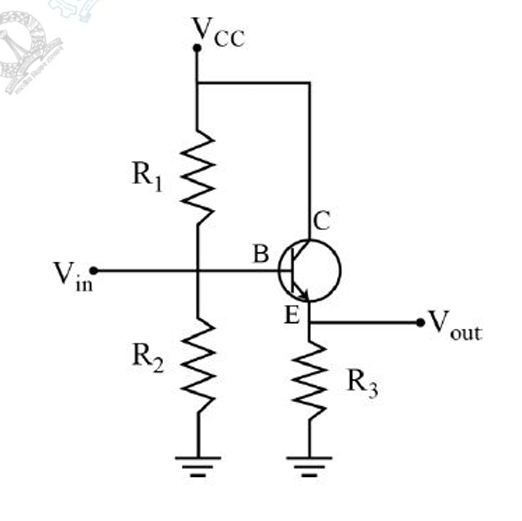
\includegraphics[width=0.3\textwidth]{figs/q52fig17.png}
\caption{transistor amplifier circuit}
\label{fig:q52}
\end{figure}
\hfill \textbf{(GATE PH 2017)}

\item Consider an ideal operational amplifier as shown in the figure below with $R_1=5$ k$\Omega$, $R_2=1$ k$\Omega$, $R_L=100$ k$\Omega$. For an applied input voltage $V=10$ mV, the current passing through $R_2$ is \underline{\hspace{3cm}} $\mu$A. (up to two decimal places).
\begin{figure}[H]
\centering
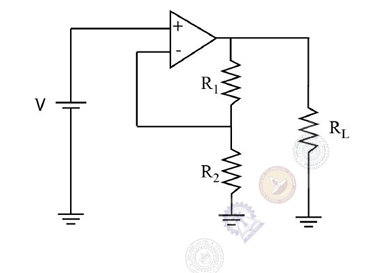
\includegraphics[width=0.45\textwidth]{figs/q53fig17.png}
\caption{ideal operational amplifier }
\label{fig:q53}
\end{figure}
\hfill \textbf{(GATE PH 2017)}

\item Consider the differential equation $\frac{dy}{dx} + y \tan(x) = \cos(x)$. If $y(0)=0$, $y(\pi/3)$ is \underline{\hspace{3cm}} (up to two decimal places).
\hfill \textbf{(GATE PH 2017)}

\item Positronium is an atom made of an electron and a positron. Given the Bohr radius for the ground state of the Hydrogen atom to be 0.53 Angstroms, the Bohr radius for the ground state of positronium is \underline{\hspace{3cm}} Angstroms. (up to two decimal places).
\hfill \textbf{(GATE PH 2017)}

\item The ninth and the tenth of this month are Monday and Tuesday \underline{\hspace{3cm}}.
\begin{enumerate}
\begin{multicols}{2}
\item figuratively
\item retrospectively
\item respectively
\item rightfully
\end{multicols}
\end{enumerate}
\hfill \textbf{(GATE PH 2017)}

\item It is \underline{\hspace{2cm}} to read this year's textbook \underline{\hspace{2cm}} the last year's.
\begin{enumerate}
\begin{multicols}{2}
\item easier, than
\item most easy, than
\item easier, from
\item easiest, from
\end{multicols}
\end{enumerate}
\hfill \textbf{(GATE PH 2017)}

\item A rule states that in order to drink beer, one must be over 18 years old. In a bar, there are 4 people. P is 16 years old, Q is 25 years old, R is drinking milkshake and S is drinking a beer. What must be checked to ensure that the rule is being followed?
\begin{enumerate}
\item Only P's drink
\item Only P's drink and S's age
\item Only S's age
\item Only P's drink, Q's drink and S's age
\end{enumerate}
\hfill \textbf{(GATE PH 2017)}

\item Fatima starts from point P, goes North for 3 km, and then East for 4 km to reach point Q. She then turns to face point P and goes 15 km in that direction. She then goes North for 6 km. How far is she from point P, and in which direction should she go to reach point P?
\begin{enumerate}
\begin{multicols}{4}
\item 8 km, East
\item 12 km, North
\item 6 km, East
\item 10 km, North
\end{multicols}
\end{enumerate}
\hfill \textbf{(GATE PH 2017)}

\item 500 students are taking one or more courses out of Chemistry, Physics, and Mathematics. Registration records indicate course enrolment as follows: Chemistry (329), Physics (186), Mathematics (295), Chemistry and Physics (83), Chemistry and Mathematics (217), and Physics and Mathematics (63). How many students are taking all 3 subjects?
\begin{enumerate}
\begin{multicols}{4}
\item 37
\item 43
\item 47
\item 53
\end{multicols}
\end{enumerate}
\hfill \textbf{(GATE PH 2017)}

\item 
\begin{quote}
“If you are looking for a history of India, or for an account of the rise and fall of the British Raj, or for the reason of the cleaving of the subcontinent into two mutually antagonistic parts and the effects this sundering will have in the respective sections, and ultimately on Asia, you will not find it in these pages; for though I have spent a lifetime in the country, I lived too near the seat of events, and was too intimately associated with the actors, to get the perspective needed for the impartial recording of these matters.”
\end{quote}
Which of the following statements best reflects the author’s opinion?
\begin{enumerate}
\item An intimate association does not allow for the necessary perspective.
\item Matters are recorded with an impartial perspective.
\item An intimate association offers an impartial perspective.
\item Actors are typically associated with the impartial recording of matters.
\end{enumerate}
\hfill \textbf{(GATE PH 2017)}

\item Each of P, Q, R, S, W, X, Y and Z has been married at most once. X and Y are married and have two children P and Q. Z is the grandfather of the daughter S of P. Further, Z and W are married and are parents of R. Which one of the following must necessarily be FALSE?
\begin{enumerate}
\item X is the mother-in-law of R
\item P and R are not married to each other
\item P is a son of X and Y
\item Q cannot be married to R
\end{enumerate}
\hfill \textbf{(GATE PH 2017)}

\item 1200 men and 500 women can build a bridge in 2 weeks. 900 men and 250 women will take 3 weeks to build the same bridge. How many men will be needed to build the bridge in one week?
\begin{enumerate}
\begin{multicols}{4}
\item 3000
\item 3300
\item 3600
\item 3900
\end{multicols}
\end{enumerate}
\hfill \textbf{(GATE PH 2017)}

\item The number of 3-digit numbers such that the digit 1 is never to the immediate right of 2 is
\begin{enumerate}
\begin{multicols}{4}
\item 781
\item 791
\item 881
\item 891
\end{multicols}
\end{enumerate}
\hfill \textbf{(GATE PH 2017)}

\item A contour line joins locations having the same height above the mean sea level. The following is a contour plot of a geographical region. Contour lines are shown at 25 m intervals in this plot.
\begin{figure}[H]
\centering
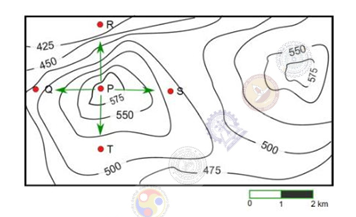
\includegraphics[width=0.6\textwidth]{figs/q65fig17.png}
\caption{contour plot of a geographical region}
\label{fig:q65}
\end{figure}
Which of the following is the steepest path leaving from P?
\begin{enumerate}
\begin{multicols}{4}
\item P to Q
\item P to R
\item P to S
\item P to T
\end{multicols}
\end{enumerate}
\hfill \textbf{(GATE PH 2017)}
    
   

\end{enumerate}

\end{document}
